\documentclass{article}

% Language setting
\usepackage[polish]{babel}

% Set page size and margins
\usepackage[a4paper,top=2cm,bottom=2cm,left=3cm,right=3cm,marginparwidth=1.75cm]{geometry}
\usepackage[T1]{fontenc}

% Useful packages
\usepackage{amsmath}
\usepackage{graphicx}
\usepackage{subcaption}
\usepackage[colorlinks=true, allcolors=blue]{hyperref}
\usepackage{float}

\title{CAD/CAE - zadanie 3}
\author{Iwo Szczepaniak}

\begin{document}
\maketitle

\section{Modyfikacje kodu źródłowego}

\subsection{Oryginalna funkcja bitmap\_h}
Pierwotna wersja kodu obsługuje wszystkie komponenty RGB jednocześnie:

\begin{verbatim}
% exctract red, green and blue components
RR = XX(:,:,1); %Red color [0,255]
GG = XX(:,:,2); %Green color [0,255]
BB = XX(:,:,3); %Blue color [0,255]
\end{verbatim}

\subsubsection{Kanał czerwony (bitmap\_h\_red)}
\begin{verbatim}
% exctract red, green and blue components
RR = XX(:,:,1); %Red color [0,255]
GG = zeros(size(XX(:,:,2)));
BB = zeros(size(XX(:,:,3)));
\end{verbatim}

\subsubsection{Kanał zielony (bitmap\_h\_green)}
\begin{verbatim}
% exctract red, green and blue components
RR = zeros(size(XX(:,:,1)));
GG = XX(:,:,2); 
BB = zeros(size(XX(:,:,3)));
\end{verbatim}

\subsubsection{Kanał niebieski (bitmap\_h\_blue)}
\begin{verbatim}
% exctract red, green and blue components
RR = zeros(size(XX(:,:,1)));
GG = zeros(size(XX(:,:,2)));
BB = XX(:,:,3);
\end{verbatim}

\section{Parametry eksperymentu}
\begin{itemize}
    \item Liczba elementów początkowych: 4x4
    \item Maksymalny błąd: 1
    \item Wrażliwość adaptacji: 1
    \item Maksymalny poziom adaptacji: zależny od możliwości sprzętowych
\end{itemize}

\section{Wyniki eksperymentów}

\subsection{Obraz oryginalny}
\begin{figure}[H]
    \centering
    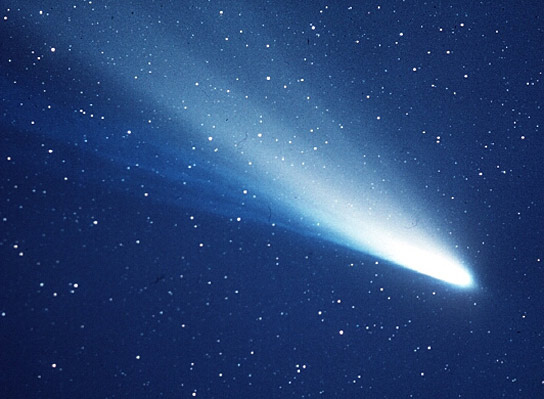
\includegraphics[width=0.8\linewidth]{halley.jpg}
    \caption{Oryginalny obraz wejściowy \hyperref[fn:source]{[1]}}
    \label{fig:original-image}
\end{figure}


\footnote[1]{\label{fn:source} Kometa Halleya: \href{https://www.tygodnikpowszechny.pl/sites/default/files/styles/art_front/public/import/1451-lamza.jpg.webp?itok=TSYe2o5i}{\text{https://www.tygodnikpowszechny.pl/sites/default/files/}\newline\text{styles/art\_front/public/import/1451-lamza.jpg.webp?itok=TSYe2o5i}}}}

\subsection{Pełna adaptacja RGB}

\begin{figure}[H]
    \centering
    \begin{subfigure}[b]{0.45\textwidth}
        \includegraphics[width=\textwidth]{Results/full_rgb/refinement_level_1.jpg}
        \caption{Wrażliwość adaptacji 1}
    \end{subfigure}
    \begin{subfigure}[b]{0.45\textwidth}
        \includegraphics[width=\textwidth]{Results/full_rgb/refinement_level_4.jpg}
        \caption{Wrażliwość adaptacji 4}
    \end{subfigure}
    \begin{subfigure}[b]{0.45\textwidth}
        \includegraphics[width=\textwidth]{Results/full_rgb/refinement_level_8.jpg}
        \caption{Wrażliwość adaptacji 8}
    \end{subfigure}
    \begin{subfigure}[b]{0.45\textwidth}
        \includegraphics[width=\textwidth]{Results/full_rgb/refinement_level_12.jpg}
        \caption{Wrażliwość adaptacji 12}
    \end{subfigure}
    \caption{Kolejne poziomy adaptacji dla pełnego RGB}
    \label{fig:full-rgb-levels}
\end{figure}

\subsection{Adaptacja kanału czerwonego}

\begin{figure}[H]
    \centering
    \begin{subfigure}[b]{0.45\textwidth}
        \includegraphics[width=\textwidth]{Results/red_channel/refinement_level_1.jpg}
        \caption{Wrażliwość adaptacji 1}
    \end{subfigure}
    \begin{subfigure}[b]{0.45\textwidth}
        \includegraphics[width=\textwidth]{Results/red_channel/refinement_level_4.jpg}
        \caption{Wrażliwość adaptacji 4}
    \end{subfigure}
    \begin{subfigure}[b]{0.45\textwidth}
        \includegraphics[width=\textwidth]{Results/red_channel/refinement_level_8.jpg}
        \caption{Wrażliwość adaptacji 8}
    \end{subfigure}
    \begin{subfigure}[b]{0.45\textwidth}
        \includegraphics[width=\textwidth]{Results/red_channel/refinement_level_12.jpg}
        \caption{Wrażliwość adaptacji 12}
    \end{subfigure}
    \caption{Kolejne poziomy adaptacji dla kanału czerwonego}
    \label{fig:red-channel-levels}
\end{figure}

\subsection{Adaptacja kanału zielonego}

\begin{figure}[H]
    \centering
    \begin{subfigure}[b]{0.45\textwidth}
        \includegraphics[width=\textwidth]{Results/green_channel/refinement_level_1.jpg}
        \caption{Wrażliwość adaptacji 1}
    \end{subfigure}
    \begin{subfigure}[b]{0.45\textwidth}
        \includegraphics[width=\textwidth]{Results/green_channel/refinement_level_4.jpg}
        \caption{Wrażliwość adaptacji 4}
    \end{subfigure}
    \begin{subfigure}[b]{0.45\textwidth}
        \includegraphics[width=\textwidth]{Results/green_channel/refinement_level_8.jpg}
        \caption{Wrażliwość adaptacji 8}
    \end{subfigure}
    \begin{subfigure}[b]{0.45\textwidth}
        \includegraphics[width=\textwidth]{Results/green_channel/refinement_level_12.jpg}
        \caption{Wrażliwość adaptacji 12}
    \end{subfigure}
    \caption{Kolejne poziomy adaptacji dla kanału zielonego}
    \label{fig:green-channel-levels}
\end{figure}

\subsection{Adaptacja kanału niebieskiego}

\begin{figure}[H]
    \centering
    \begin{subfigure}[b]{0.45\textwidth}
        \includegraphics[width=\textwidth]{Results/blue_channel/refinement_level_1.jpg}
        \caption{Wrażliwość adaptacji 1}
    \end{subfigure}
    \begin{subfigure}[b]{0.45\textwidth}
        \includegraphics[width=\textwidth]{Results/blue_channel/refinement_level_4.jpg}
        \caption{Wrażliwość adaptacji 4}
    \end{subfigure}
    \begin{subfigure}[b]{0.45\textwidth}
        \includegraphics[width=\textwidth]{Results/blue_channel/refinement_level_8.jpg}
        \caption{Wrażliwość adaptacji 8}
    \end{subfigure}
    \begin{subfigure}[b]{0.45\textwidth}
        \includegraphics[width=\textwidth]{Results/blue_channel/refinement_level_12.jpg}
        \caption{Wrażliwość adaptacji 12}
    \end{subfigure}
    \caption{Kolejne poziomy adaptacji dla kanału niebieskiego}
    \label{fig:blue-channel-levels}
\end{figure}

\end{document}